\documentclass{article}
\usepackage{tkz-graph}
\usepackage{paralist}
\pagestyle{empty}
\usetikzlibrary{patterns}

\begin{document}

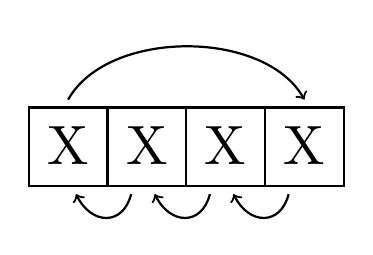
\begin{tikzpicture}

\draw[thick] (0,0) rectangle (1,1);
\draw[thick] (1,0) rectangle (2,1);
\draw[thick] (2,0) rectangle (3,1);
\draw[thick] (3,0) rectangle (4,1);

\draw (0.5,1) node[anchor=north, scale=2] {X};
\draw (1.5,1) node[anchor=north, scale=2] {X};
\draw (2.5,1) node[anchor=north, scale=2] {X};
\draw (3.5,1) node[anchor=north, scale=2] {X};

\draw[thick,->] (0.5,1.1) .. controls (1,2) and (3,2) .. (3.5,1.1);
\draw[thick,<-] (0.6,-0.1) .. controls (0.8,-0.5) and (1.2,-0.5) .. (1.3,-0.1);
\draw[thick,<-] (1.6,-0.1) .. controls (1.8,-0.5) and (2.2,-0.5) .. (2.3,-0.1);
\draw[thick,<-] (2.6,-0.1) .. controls (2.8,-0.5) and (3.2,-0.5) .. (3.3,-0.1);

\end{tikzpicture}

\end{document}